\documentclass[conference]{IEEEtran}
\IEEEoverridecommandlockouts
\usepackage{amsmath,amssymb}
\usepackage{graphicx}
\usepackage{booktabs}
\usepackage[table]{xcolor}
\usepackage{url}
\usepackage{cite}
\usepackage{balance}
\usepackage{pifont}
\usepackage[most]{tcolorbox}
\newcommand{\cmark}{\ding{51}}
\newcommand{\pmark}{$\circ$}
\makeatletter\newcommand{\settabcaptype}{\def\@captype{table}}\makeatother
\definecolor{navy}{HTML}{1B2A4A}
\definecolor{boxbg}{HTML}{EEF3FA}
\newtcolorbox{findings}[1]{enhanced,colback=boxbg,colframe=navy,boxrule=0.6pt,arc=1.5pt,left=3pt,right=3pt,top=2pt,bottom=2pt,
  fonttitle=\bfseries\footnotesize,title=#1,fontupper=\footnotesize}
\graphicspath{{figures/}}
\newcommand{\XgbRaw}{0.020}
\newcommand{\XgbCal}{0.010}
\newcommand{\XgbAUC}{0.626}
\newcommand{\XgbPR}{0.122}
\newcommand{\LrAUC}{0.666}
\newcommand{\LrPR}{0.150}
\newcommand{\DtRaw}{0.037}
\newcommand{\DtCal}{0.011}
\newcommand{\TestPrev}{7.4}
\newcommand{\TestRows}{3,000}
\newcommand{\GapTwo}{2.1}
\newcommand{\GapThree}{10.8}
\newcommand{\BizNone}{116.9}
\newcommand{\BizCal}{118.3}
\newcommand{\BizUncal}{120.4}
\newcommand{\BizOracle}{82.1}
\newcommand{\BizAll}{664.3}
\newcommand{\PolAlerts}{5}
\newcommand{\PolTP}{0}
\newcommand{\LinkSel}{MLP}
\newcommand{\LinkSelAP}{0.227}
\newcommand{\LinkBase}{0.117}
\newcommand{\LinkSAGEAP}{0.168}
\newcommand{\LinkSelP}{0.32}
\newcommand{\LinkCand}{8,863}
\newcommand{\LinkHid}{1,039}
\newcommand{\DcXgbAUC}{0.780}
\newcommand{\DcXgbPR}{0.858}
\newcommand{\DcBaseAUC}{0.744}
\newcommand{\DcRegR}{0.27}
\newcommand{\DcBaseR}{0.28}
\newcommand{\DcTest}{34,554}
\newcommand{\SevA}{4.72}
\newcommand{\SevB}{3.98}
\newcommand{\SevC}{1.16}
\newcommand{\SaveAC}{3.56}
\newcommand{\SaveACl}{3.25}
\newcommand{\SaveACh}{3.87}
\newcommand{\SaveBC}{2.82}
\newcommand{\SaveAB}{0.74}
\newcommand{\SevUnmetA}{734}
\newcommand{\SevUnmetB}{605}
\newcommand{\SevUnmetC}{39}
\newcommand{\SevSvcA}{64}
\newcommand{\SevSpendC}{4.62}
\newcommand{\ModExtraC}{-16.7}
\newcommand{\MildExtraC}{0.82}
\newcommand{\ModSaveAC}{16.7}
\newcommand{\ModA}{61.5}
\newcommand{\ModB}{50.5}
\newcommand{\ModC}{44.8}
\newcommand{\SevRed}{75}
\newcommand{\FullRecC}{88}
\newcommand{\Reps}{500}
\newcommand{\Censored}{3}
\newcommand{\ModAWins}{82}
\newcommand{\SevCWins}{73}
\newcommand{\HubObs}{19}
\newcommand{\HubHid}{25}
\newcommand{\McSE}{3.9}
\newcommand{\CiLrRoc}{0.626--0.705}
\newcommand{\CiXgbRoc}{0.587--0.664}
\newcommand{\CiLrPr}{0.117--0.192}
\newcommand{\CiXgbPr}{0.099--0.155}
\newcommand{\DRoc}{0.040}
\newcommand{\DRocP}{0.008}
\newcommand{\DEce}{0.0095}
\newcommand{\DEceL}{-0.002}
\newcommand{\DEceH}{0.020}
\newcommand{\DEceP}{0.11}
\newcommand{\DcCi}{0.775--0.784}
\newcommand{\DcDelta}{0.035}
\newcommand{\SensSevC}{1.17}
\newcommand{\SensSaveAC}{3.67}
\newcommand{\SensModC}{45.7}

\begin{document}

\title{Supply Chain Black Box: Hidden Supplier Dependency Discovery, Calibrated Cascading-Risk Prediction and Optimised Recovery for an FMCG Manufacturer}

\author{\IEEEauthorblockN{Shraddha Shete, Shirsodeep Biswas, Jayant Kumawat}
\IEEEauthorblockA{\textit{Goa Institute of Management} -- Big Data Analytics\\
Student IDs: \{B2026102, B2026100, B2026078\}\\
\{shraddha.shete2026b, shirsodeep.biswas2026b, jayant.kumawat2026b\}@gim.ac.in}}

\maketitle

\begin{abstract}
A fast-moving consumer goods (FMCG) manufacturer of chocolate and malt beverages sees its Tier-1 suppliers but not the Tier-2/3 suppliers they share. In a documented
\emph{synthetic} supply network (500 suppliers, 69\,\% of links hidden) we test whether ranked estimates of hidden links improve recovery
decisions. The system predicts supplier disruption, ranks candidate hidden links, simulates cascades and plans recovery with a mixed-integer linear
program (MILP); two real datasets check transferable components only. Observed links
understate Tier-2/3 exposure \GapTwo$\times$/\GapThree$\times$; logistic regression out-ranks the pre-specified XGBoost model; the calibration gain is not significant and
graph neural networks did not beat tabular models. In 500 paired simulations of a severe outage of the five largest cocoa traders, the
optimisation policy lowers simulated impact from \SevA{} to \SevC{} crore Indian rupees (INR). A factorial ablation attributes most of this to the predicted
links: with the same MILP, the observed graph alone gives \AblCobs{} crore. For mild shocks doing nothing is cheapest in all \SensN{} sensitivity
settings. All monetary results are simulated and assumption-conditional, not estimates of real-world savings.
\end{abstract}

\begin{IEEEkeywords}
supply chain risk, link prediction, probability calibration, cascading disruption, recovery optimisation, ablation, FMCG
\end{IEEEkeywords}

\section{Introduction}
\subsection{Business Problem}
Disruptions are followed by significantly lower long-run stock returns~\cite{hendricks2005}. Each Tier-1 input of a malt beverage (malt,
milk powder, cocoa, sugar, packaging) depends on Tier-2 traders that procurement rarely maps, so shocks ripple through invisible links~\cite{ivanov2019}. Fig.~\ref{fig:arch} shows the system that supports two decisions: \emph{(D1) each month, which mitigation action to take for each supplier;
(D2) when a shock is reported, which alternates receive which quantities, by which transport mode.}

\subsection{Related Work, Novelty and Provenance}
\textbf{Search.} A targeted (not systematic) search on 13 Nov 2026 of a web search engine, RePEc/IDEAS, SSRN and arXiv used the terms
hidden-link prediction, deep-tier visibility, disruption mitigation optimisation and supplier disruption prediction. \textbf{Closest work} (Table~\ref{tab:prior}): link prediction recovers hidden
supplier links~\cite{brintrup2018,kosasih2022}; deep-tier \emph{true} visibility improves simulated resilience assessment~\cite{taghizadeh2021};
machine learning (ML) predicts first-tier disruption~\cite{brintrup2020}; graph neural networks (GNNs) are benchmarked on SupplyGraph~\cite{wasi2024}; operations research/management science (OR/MS) and ripple-effect work
models mitigation and propagation~\cite{snyder2016,ivanov2019}; few AI studies reach the response stage~\cite{baryannis2019}. \textbf{Differentiator.} We found no study that feeds \emph{predicted} (uncertain) links into a recovery optimiser
and separates their value from the optimiser's by comparing observed-graph, predicted-graph and true-graph arms under identical conditions.
The contribution is systems integration plus a controlled synthetic decision experiment, not new methods or real-world savings.
\textbf{Provenance} (author declaration): built in the public repository from 12~Nov~2026 (dated git history); no earlier project of the authors was reused.

\begin{table}[t]\centering\caption{Scope of related work. \cmark{} = primary focus; \pmark{} = partial coverage or review; blank = not addressed.
HL hidden-link prediction; RP risk prediction; CA calibration; CS cascade propagation; RO recovery optimisation; PE policy evaluation.}\label{tab:prior}
\scriptsize\setlength{\tabcolsep}{3.2pt}\begin{tabular}{@{}lcccccc@{}}\toprule
Work & HL & RP & CA & CS & RO & PE\\\midrule
Brintrup \emph{et al.} 2018~\cite{brintrup2018} & \cmark & & & & & \\
Kosasih \& Brintrup 2022~\cite{kosasih2022} & \cmark & & & & & \\
Brintrup \emph{et al.} 2020~\cite{brintrup2020} & & \cmark & & & & \\
Wasi \emph{et al.} 2024~\cite{wasi2024} & & \cmark & & & & \\
Taghizadeh \emph{et al.} 2021~\cite{taghizadeh2021} & \pmark & & & \cmark & & \cmark\\
Snyder \emph{et al.} 2016~\cite{snyder2016} & & & & \pmark & \cmark & \pmark\\
Ivanov \emph{et al.} 2019~\cite{ivanov2019} & & \pmark & & \cmark & & \\
Baryannis \emph{et al.} 2019~\cite{baryannis2019} & & \pmark & & & \pmark & \\
\rowcolor{gray!15}\textbf{This work (synthetic)} & \cmark & \cmark & \cmark & \cmark & \cmark & \cmark\\
\bottomrule\end{tabular}\end{table}

\subsection{Research Questions, Hypotheses and Map}
\textbf{RQ1/H1}: point-in-time features give above-chance 30-day risk ranking, and calibration lowers ECE (expected calibration error).
\textbf{RQ2/H2}: the observed network understates upstream exposure, and link prediction ranks hidden links above the base rate in average precision (AP).
\textbf{RQ3/H3}: GNNs beat tabular models. \textbf{RQ4a/H4a}: the optimisation policy C has lower expected impact than
rule-based B and no intervention A \emph{at every severity}. \textbf{RQ4b/H4b}: holding the MILP fixed, adding predicted links lowers impact.
Table~\ref{tab:map} links each question to its experiment and verdict.

\begin{table}[t]\centering\caption{Research map. E3 is a separate shipment-lateness task on real data; it does not validate the supplier-risk model.}\label{tab:map}
\scriptsize\setlength{\tabcolsep}{1.8pt}\begin{tabular}{@{}lllll@{}}\toprule
RQ & Exp.\ (data) & Test & Verdict & Output used in\\\midrule
1 & E1 (synthetic) & bootstrap & partly & D1 action; MILP screen\\
2 & E2A (synthetic) & AP vs.\ base & supported & exposure; C's graph\\
3 & E2B (synth.+real) & 5 seeds & not supported & model choice\\
-- & E3 (DataCo, real) & bootstrap & transfer only & lateness API\\
4a & S1--S9 (simulated) & Wilcoxon--Holm & not supported & tiered policy\\
4b & Ablation (simul.) & Wilcoxon--Holm & severe only & novelty claim\\
\bottomrule\end{tabular}\end{table}

\begin{figure*}[t]\centering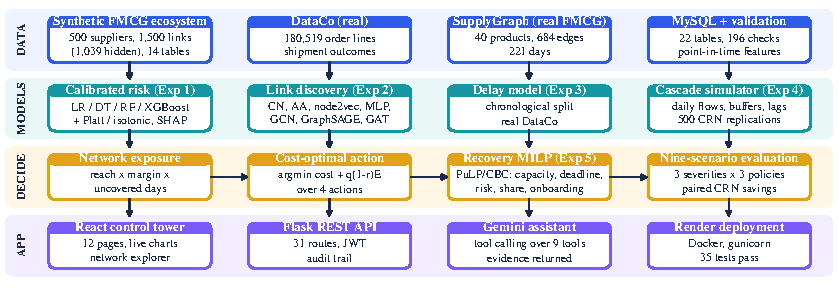
\includegraphics[width=0.74\textwidth]{fig_architecture.pdf}
\caption{System architecture. Real and synthetic data feed point-in-time features; risk, link, delay and cascade models feed an exposure model,
a cost-based action rule and a recovery MILP, served by a Flask API, a React control tower and a tool-calling Gemini assistant (Render).}\label{fig:arch}\end{figure*}

\section{Methodology}
\subsection{Data, Units and Provenance}
\textbf{Synthetic ecosystem} (fictional, seed 42): 120/200/180 Tier-1/2/3 suppliers, 50 materials, 100 products, two plants, 1,048 disruptions
(782 qualifying) in 2024--2025. A buyer of material $m$ picks $k\in\{2,\dots,6\}$ sources with probability $\propto$ size$^{1.6}e^{-d/2500\,\mathrm{km}}$;
Tier-2/3 links are visible with probability 0.45/0.15 (461 of 1,500 observed). Disruption hazards include contagion over the \emph{true} network; hidden links serve only as ground truth.
\textbf{DataCo}~\cite{constante2019} (real, CC~BY~4.0; the Mendeley V5 file obtained from a pinned public mirror and SHA-256 checked): 180,519 order lines, 7,754 cancelled removed; it has no supplier
identities. \textbf{SupplyGraph}~\cite{wasi2024} (real FMCG): 40 products, 684 edges, 221 days.  The synthetic tables pass 178 automated validation checks. Money is INR; 1~lakh (L) = $10^5$ and 1~crore (Cr) = $10^7$ INR.

\subsection{Disruption Prediction and Leakage Control (RQ1)}
The prediction timestamp $t$ is 00:00 on the first of each month. For supplier $i$,
\begin{equation}\label{eq:label}
y_i(t)=\mathbb{1}\big[\exists e:\ s_e\in(t,t+30\mathrm{d}],\ \ell_e\ge0.25,\ d_e\ge3\big],
\end{equation}
with start $s_e$, capacity loss $\ell_e$ and duration $d_e$ (days). The 25 features use only information available before $t$ and \emph{observed}
links. Splits: train 2024-04..2025-02 (5,500 supplier-months), one-month embargo, calibration 2025-04..06 (1,500), test 2025-07..12 (\TestRows).
Logistic regression (LR), a decision tree, a random forest and XGBoost~\cite{chen2016} are compared by the area under the ROC curve (ROC-AUC), the area under the precision--recall curve (PR-AUC), the Brier score and ECE; Platt scaling~\cite{platt1999} and isotonic
regression~\cite{zadrozny2002,niculescu2005} are fitted on the calibration split; the method is chosen by 5-fold cross-validated Brier score
\emph{within} that split, never on test data. XGBoost was fixed as the primary model in the code before any result was seen; its Platt-calibrated
probability $q_i$ feeds D1, the MILP risk screen and the simulated failure chance of alternates.

\subsection{Link Prediction and Graph Models (RQ2, RQ3)}
The graph has 501 nodes: 500 suppliers and the manufacturer; supplier-level results use the 500 suppliers. \emph{Link prediction} scores
candidate pairs; \emph{hidden-link discovery} evaluates those scores against the synthetic ground truth. \textbf{A1}: observed links split
70/10/20 with test links removed from message passing. Comparators: heuristics~\cite{libennowell2007}, node2vec~\cite{grover2016}, a multilayer perceptron (MLP) and GNNs. \textbf{A2}: rank all \LinkCand{} material-compatible unobserved pairs against
\LinkHid{} hidden links; the model is chosen by validation AP. \textbf{E2B} feeds E1 features through GCN~\cite{kipf2017}, GraphSAGE~\cite{hamilton2017} and
GAT~\cite{velickovic2018} on observed, observed+top-500 predicted and true graphs, and predicts a 7-day shortfall on SupplyGraph.

\subsection{Exposure, Simulation and Decision Rule (D1)}
Exposure $E_i$ (INR) is the expected contribution-margin loss at the manufacturer if supplier $i$ is disrupted (CM = contribution margin):
\begin{equation}\label{eq:exposure}
E_i=\textstyle\sum_m r_{im}\,\mathrm{CM}_m\,\mathbb{E}\big[S\max(0,D-c_m-10(\tau_i-1))\big],
\end{equation}
with reach $r_{im}$ (product of dependency shares along paths), daily contribution margin $\mathrm{CM}_m$, cover $c_m$ (days), tier $\tau_i$ and
empirical severity/duration $(S,D)$. The simulator propagates availability daily over the true network. The action is $a^*=\arg\min_a C_a+q_i(1-\rho_a)E_i$ over four actions with cost $C_a$ = 0/5k/20k/60k INR and
assumed risk reduction $\rho_a$ = 0/0.15/0.45/0.70; it is Bayes-optimal only if $q_i$ is calibrated, with break-even $q^*=\Delta C/(E_i\Delta\rho)$.

\subsection{Recovery MILP, Scenarios and Robustness Design (RQ4)}
For deficits $\delta_m$ the MILP (PuLP/CBC) chooses quantities $x_{jk}$ from candidate $j$ by mode $k$, onboarding $z_j$ and shortage $s_m$:
\begin{align}
\min\ &\textstyle\sum_{jk}p_j(1+f_{jk}+hW/2)x_{jk}+\sum_jFz_j+\sum_m\pi_ms_m\\
\text{s.t. }&\textstyle\sum_{jk}\rho_j(1-q_j)\kappa_j\alpha_jx_{jk}+s_m\ge\delta_m,\nonumber\\
&x_{jk}\le u_j(W-L_{jk})^+,\ \ \textstyle\sum_kx_{jk}\le0.6\,\delta_m,\ \ q_j\le0.35,\nonumber
\end{align}
with price $p_j$, freight $f_{jk}$, holding rate $h$, deadline $W$, onboarding cost $F$, penalty $\pi_m$, compatibility $\kappa_j$, spare capacity
$u_j$ and availability $\alpha_j$ de-rated by estimated dependency on the disrupted suppliers. The shock removes 25/50/100\,\% of the capacity of
the five largest Tier-2 cocoa traders for a nominal 60 days. \textbf{A} does nothing; \textbf{B} uses the observed graph, excludes any alternate
linked to the failed traders and allocates by reliability when cover falls below 10 days; \textbf{C} uses the observed+predicted graph and the
MILP at detection plus the same trigger. All arms share network, demand, inventory and illustrative economics, and replication $r$ uses seed
$s_0+r$ for every arm (common random numbers, CRN; 180-day horizon). \textbf{Ablation (RQ4b):} a $2\times2$ factorial \{rule, MILP\}$\times$\{observed,
observed+predicted graph\} plus an oracle arm (MILP, true graph) isolates the value of predicted links. \textbf{Sensitivity:} one at a time, we
vary management overhead, shortage penalty, interruption cost, duration, alternates' spare capacity and failure risk, and how many links the
buyer knows (200 CRN replications per cell).

\subsection{Statistical Analysis}
Bootstraps ($B$=1,000, percentile confidence intervals (CIs), two-sided) resample suppliers in E1 (their months are dependent) and orders in E3. Policies: the estimand is the mean paired saving
$\Delta$ = impact(first) $-$ impact(second), so $\Delta>0$ means the second arm is cheaper; we report a bootstrap CI of the mean, the median,
the share of replications in which the second arm is cheaper, and a two-sided Wilcoxon signed-rank test, Holm-adjusted within each family
(9 policy comparisons; 12 ablation comparisons). $\alpha$=0.05. Policies, shock, 13 outcome metrics, CRN and replication count were fixed before any scenario run.

\section{Results}
\begin{figure*}[t]\centering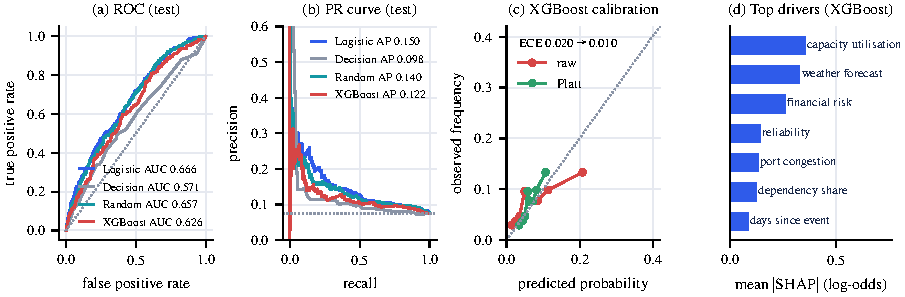
\includegraphics[width=0.8\textwidth]{fig_exp1.pdf}
\caption{E1 on the untouched test split (3,000 supplier-months, synthetic): (a) ROC and (b) precision--recall of the four calibrated models,
(c) XGBoost reliability before/after Platt scaling, (d) mean absolute SHAP (SHapley Additive exPlanations) value of the top XGBoost features.}\label{fig:exp1}\end{figure*}

\begin{table}[t]\centering\caption{E1: 30-day supplier disruption prediction on the untouched test split (3,000 supplier-months, prevalence 7.4\%). AUCs after Platt scaling (rank-preserving); calibrators fitted on the calibration split only; bold = lowest ECE per model; shaded = pre-specified primary model. 95\% CIs and tests in Table~\ref{tab:stats}.}\label{tab:exp1}
\scriptsize\setlength{\tabcolsep}{2.4pt}\begin{tabular}{@{}lcccccccc@{}}\toprule
 & & & \multicolumn{2}{c}{Brier} & \multicolumn{3}{c}{ECE$_{10}$}\\\cmidrule(lr){4-5}\cmidrule(lr){6-8}
Model & ROC-AUC & PR-AUC & raw & Platt & raw & Platt & Iso.\\\midrule
Logistic reg. & 0.666 & 0.150 & 0.0669 & 0.0670 & 0.0066 & \textbf{0.0059} & 0.0070\\
Decision Tree & 0.571 & 0.098 & 0.0704 & 0.0689 & 0.0366 & \textbf{0.0111} & 0.0124\\
Random Forest & 0.657 & 0.140 & 0.0672 & 0.0675 & \textbf{0.0046} & 0.0081 & 0.0063\\
\rowcolor{gray!15}XGBoost & 0.626 & 0.122 & 0.0689 & 0.0680 & 0.0197 & \textbf{0.0104} & 0.0109\\
\bottomrule\end{tabular}\end{table}
\begin{table}[t]\centering\caption{Statistical tests. E1: supplier-cluster bootstrap ($B$=1,000, 500 suppliers, 3,000 test months); E3: order-line bootstrap ($B$=1,000); S: 500 paired CRN replications, 95\% CI of the mean saving and Wilcoxon signed-rank $p$, Holm-adjusted over nine comparisons. Win = share of replications in which the second policy is cheaper (L = INR lakh).}\label{tab:stats}
\scriptsize\setlength{\tabcolsep}{2pt}\begin{tabular}{@{}llrccr@{}}\toprule
 & Comparison & Effect & 95\% CI & Win & $p$\\\midrule
E1 & LR $-$ XGBoost, ROC-AUC & +0.040 & [0.013, 0.068] & -- & 0.008\\
E1 & LR $-$ XGBoost, PR-AUC & +0.026 & [0.002, 0.055] & -- & 0.044\\
E1 & ECE reduction, XGB raw $-$ Platt & +0.0095 & [-0.0018, 0.0197] & -- & 0.108\\
E3 & XGBoost $-$ mode baseline, ROC-AUC & +0.035 & [0.032, 0.039] & -- & $<$0.001\\
\midrule
S & Severe: saving of C over A (L) & +356.2 & [324.9, 387.4] & 80\% & $<$0.001\\
S & Severe: saving of C over B (L) & +282.0 & [252.7, 311.4] & 73\% & $<$0.001\\
S & Moderate: saving of C over A (L) & +16.7 & [9.1, 24.3] & 17\% & $<$0.001\\
S & Moderate: saving of B over A (L) & +11.0 & [8.7, 13.3] & 18\% & 0.167\\
S & Mild: saving of C over A (L) & -0.8 & [-0.8, -0.8] & 0\% & $<$0.001\\
\bottomrule\end{tabular}\end{table}
\subsection{Disruption Prediction (RQ1: partly supported)}
Ranking is modest (prevalence \TestPrev\,\%; Table~\ref{tab:exp1}, Fig.~\ref{fig:exp1}). Logistic regression is best (ROC-AUC \LrAUC, 95\,\% CI \CiLrRoc; PR-AUC
\LrPR) and significantly better than XGBoost (\XgbAUC, CI \CiXgbRoc; Table~\ref{tab:stats}); validation data also favoured it. We keep
XGBoost to avoid test-set model choice; using logistic-regression risk moves severe C impact only from \SevC{} to \SensSevC{} Cr. Platt scaling lowered XGBoost's ECE from \XgbRaw{} to \XgbCal, not significantly ($p$=\DEceP); it helped the
decision tree (\DtRaw$\rightarrow$\DtCal) and worsened the already-calibrated random forest. D1 probabilities rank above chance but are not shown to be operationally calibrated.
On the test months the cost rule raised \PolAlerts{} alerts, none followed by a qualifying
disruption; realised cost (\BizCal{} L) was close to monitor-only (\BizNone{} L). This is a small retrospective demonstration, not validation.

\begin{figure*}[t]\centering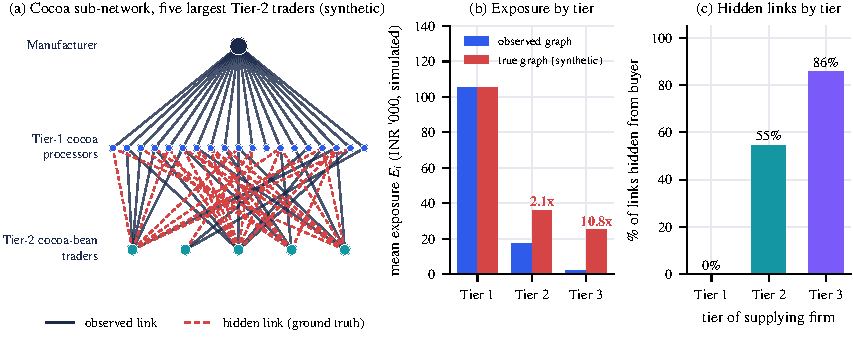
\includegraphics[width=0.78\textwidth]{fig_blackbox.pdf}
\caption{The black-box gap in the synthetic network: (a) cocoa sub-network---dashed links exist in the synthetic ground truth but are hidden
from the buyer; (b) mean exposure $E_i$ (expected margin loss, Eq.~\eqref{eq:exposure}) per supplier on the observed vs.\ true graph; (c) share of hidden links by tier.}\label{fig:gap}\end{figure*}

\subsection{Exposure Gap and Link Prediction (RQ2: supported; RQ3: not supported)}
Observed links understate Tier-2/3 exposure \GapTwo$\times$/\GapThree$\times$ (Fig.~\ref{fig:gap}). This measures exposure, not prediction. The validation-selected \LinkSel{} pair model reaches AP \LinkSelAP{} (mean of five seeds) against a base rate of \LinkBase{} (precision
\LinkSelP{} in its top 100; Table~\ref{tab:exp2a}); the single ranked list passed to the simulator (seed 0) has AP 0.220. This is useful ranking inside this synthetic candidate set, not proof that recovered links are real
suppliers. GNNs did not improve risk classification: on synthetic data the best GNN reaches PR-AUC 0.111$\pm$0.011 (observed+predicted graph) and 0.108 with the true graph vs.\ 0.122 for XGBoost; on real SupplyGraph logistic regression (0.488) beats the best GNN (0.461$\pm$0.017; 5 seeds).

\begin{table}[t]\centering\caption{E2A link prediction (synthetic, 5 seeds for learned models). A1: held-out observed edges vs.\ material-compatible negatives. A2: ranking all 8,863 compatible unobserved pairs against 1,039 ground-truth hidden edges (base rate 0.117). Learned models: mean$\pm$sd over 5 seeds; the seed-0 MLP list used downstream has AP 0.220 and P@100 0.29. Adamic--Adar equals common neighbours. P@100/R@500 = precision of top 100/recall of top 500.}\label{tab:exp2a}\scriptsize\setlength{\tabcolsep}{2.6pt}\begin{tabular}{lccccc}\toprule
 & \multicolumn{2}{c}{A1 (held-out)} & \multicolumn{3}{c}{A2 (hidden-edge discovery)}\\\cmidrule(lr){2-3}\cmidrule(lr){4-6}
Method & ROC-AUC & AP & AP & P@100 & R@500\\\midrule
Common neigh. & 0.500 & 0.500 & 0.117 & 0.06 & 0.042 \\
Pref.~attach. & 0.733 & 0.763 & 0.166 & 0.34 & 0.120 \\
Node2Vec & 0.638 & 0.609 & 0.146 & 0.24 & 0.084 \\
MLP & 0.826$\pm$0.017 & 0.849$\pm$0.012 & 0.227$\pm$0.010 & 0.32 & 0.141 \\
GCN & 0.807$\pm$0.020 & 0.837$\pm$0.010 & 0.176$\pm$0.007 & 0.25 & 0.109 \\
GraphSAGE & 0.737$\pm$0.009 & 0.784$\pm$0.012 & 0.168$\pm$0.005 & 0.29 & 0.102 \\
GAT & 0.796$\pm$0.005 & 0.811$\pm$0.018 & 0.177$\pm$0.008 & 0.26 & 0.103 \\
\bottomrule\end{tabular}\end{table}
\subsection{Transfer to Real Shipments (DataCo)}
On \DcTest{} chronologically held-out order lines (\DcOrders{} orders) XGBoost reaches ROC-AUC \DcXgbAUC{} (CI \DcCi; PR-AUC \DcXgbPR) vs.\
\DcBaseAUC{} for a shipping-mode baseline ($+$\DcDelta, $p<$0.001); delay-days regression adds nothing ($R^2$ \DcRegR{} vs.\ \DcBaseR). This is a separate lateness task; it does not validate the network-level results.

\subsection{Executable Decision Example (D1, D2)}
For supplier S0065 (Tier-1) at $t$=2025-12-01, XGBoost gives 40.8\,\% raw and 15.2\,\% calibrated risk and $E_i$ = INR 4.41~L; with
break-even thresholds of 7.6/11.3/36.3\,\%, expected costs are 66.9/61.9/56.8/80.1 thousand INR, so a contingency review is chosen, and the
MILP returns an optimal standby plan (INR 15.1k). This shows traceability, not that the rule improves outcomes.

\begin{figure*}[!tp]\centering
{\renewenvironment{table*}[1][]{\settabcaptype}{}\begin{table*}[t]\centering\caption{Nine-scenario evaluation (means of 500 common-random-number replications; simulated INR on synthetic data). Severity = capacity loss of the five largest Tier-2 cocoa-bean traders for a nominal 60 days (log-normal). Policy A none, B rule-based, C optimisation. Disrupted capacity available: 75\,\% / 50\,\% / 0\,\% for all policies.}\label{tab:scen}
\scriptsize\setlength{\tabcolsep}{3pt}\begin{tabular}{lllrrrrrrlrrr}\toprule
Scen. & Sev. & Pol. & Aff.\ sup. & Aff.\ mat. & Unmet (k units) & Inv.\ short.\ (L) & Procure.\ (L) & Transport (L) & Impact, Cr [95\% PI] & Recov.\ d & Alt.\ util.\ \% & Full rec.\ \%\\\midrule
S1 & Mil. & A & 10.4 & 2.4 & 0.0 & 0.0 & 0.0 & 0.00 & 0.24 [0.00, 0.30] & 93 & 0 & 100\\
S2 & Mil. & B & 10.4 & 2.4 & 0.0 & 0.0 & 0.0 & 0.00 & 0.24 [0.00, 0.30] & 93 & 0 & 100\\
S3 & Mil. & C & 10.4 & 2.4 & 0.0 & 0.0 & 4.7 & 0.12 & 0.24 [0.01, 0.31] & 93 & 7 & 100\\\midrule
S4 & Mod. & A & 17.3 & 4.0 & 1.1 & 0.1 & 0.0 & 0.00 & 0.29 [0.24, 0.43] & 114 & 0 & 94\\
S5 & Mod. & B & 17.3 & 4.0 & 1.1 & 0.1 & 0.0 & 0.00 & 0.29 [0.24, 0.43] & 114 & 1 & 94\\
S6 & Mod. & C & 17.3 & 3.7 & 0.0 & 0.0 & 85.0 & 2.91 & 0.40 [0.36, 0.41] & 113 & 26 & 100\\\midrule
S7 & Sev. & A & 19.9 & 4.0 & 586.2 & 36.6 & 0.0 & 0.00 & 3.73 [0.24, 7.65] & 115 & 0 & 10\\
S8 & Sev. & B & 19.9 & 4.0 & 462.5 & 29.6 & 9.3 & 0.37 & 3.02 [0.25, 7.10] & 115 & 32 & 11\\
S9 & Sev. & C & 19.9 & 3.8 & 0.0 & 0.0 & 442.8 & 23.52 & 0.87 [0.82, 0.90] & 115 & 35 & 100\\
\bottomrule\end{tabular}\end{table*}}\par\vspace{4pt}
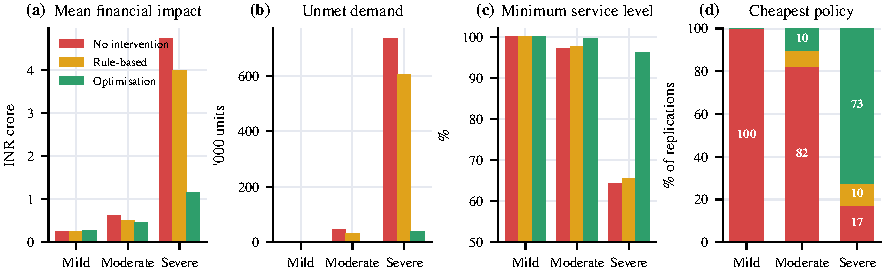
\includegraphics[width=0.8\textwidth]{fig_scenarios.pdf}
\caption{Simulated outcomes on the synthetic supply network across mild, moderate and severe disruption scenarios (500 common-random-number replications): (a) mean financial impact in INR crore; (b) unmet demand in thousand units; (c) minimum service level achieved; and (d) percentage of replications in which each policy is the cheapest. Error bars in (a) and (b): 95\,\% CI of the mean.}\label{fig:scen}\end{figure*}

\subsection{Nine-Scenario Evaluation (RQ4a: not supported overall)}\label{sec:scen}
Table~\ref{tab:scen} and Fig.~\ref{fig:scen} summarise the nine scenarios; Table~\ref{tab:stats} gives the tests. \emph{Severe}: A leaves \SevUnmetA{}k units unmet (\SevA{} Cr), B \SevUnmetB{}k (\SevB{} Cr) and C \SevUnmetC{}k (\SevC{} Cr). C saves
\SaveAC{} Cr over A (95\,\% CI \SaveACl--\SaveACh; median \SevACmed{} Cr) and is cheaper in \SevACwin\,\% of replications.
\emph{Moderate}: C saves \ModSaveAC{} L over A on the mean, yet in the median replication C costs \ModACmed{} L \emph{more} and is cheaper in
only \ModACwin\,\%; the significant Wilcoxon test reflects that typical shift against C, while the mean is driven by rare long outages.
\emph{Mild}: impact is mostly assumed management overhead; C costs \MildExtraC{} L more than A in every replication (small spread: only its
pre-booked orders differ). H4a is therefore not supported; C is preferable only for severe shocks.

\begin{table}[t]\centering\caption{Link-information ablation (RQ4b). Mean simulated impact, INR lakh $\pm$ 95\% CI (500 CRN replications); only logic or known graph changes. Lower block: paired saving, mean/median, Holm-adjusted Wilcoxon $p$ over 12 comparisons.}\label{tab:abl}
\scriptsize\setlength{\tabcolsep}{2.2pt}\begin{tabular}{@{}lllrrr@{}}\toprule
Arm & Logic & Graph known & Mild & Moderate & Severe\\\midrule
A & -- & -- & 25.7$\pm$1.2 & 61.5$\pm$8.6 & 472.1$\pm$35.7\\
B-obs & rule & observed & 25.7$\pm$1.2 & 50.5$\pm$6.8 & 398.0$\pm$33.9\\
B-pred & rule & obs.+pred. & 25.7$\pm$1.2 & 62.0$\pm$8.6 & 472.6$\pm$35.7\\
C-obs & MILP & observed & 25.7$\pm$1.2 & 48.6$\pm$6.4 & 363.6$\pm$32.1\\
C-pred = C & MILP & obs.+pred. & 26.5$\pm$1.2 & 44.8$\pm$1.3 & 115.9$\pm$6.6\\
C-oracle & MILP & true & 25.7$\pm$1.2 & 38.3$\pm$2.1 & 120.7$\pm$8.1\\\midrule
\multicolumn{3}{@{}l}{Links, MILP: C-obs$-$C} & -0.8/-0.8 & +3.9/-11.7 & +247.7/+148.5\\
\multicolumn{3}{@{}r}{\textit{$p_{\mathrm{Holm}}$}} & $<$.001 & $<$.001 & $<$.001\\
\multicolumn{3}{@{}l}{Links, rule: B-obs$-$B-pred} & +0.0/+0.0 & -11.5/-0.5 & -74.6/-93.8\\
\multicolumn{3}{@{}r}{\textit{$p_{\mathrm{Holm}}$}} & .109 & $<$.001 & $<$.001\\
\multicolumn{3}{@{}l}{MILP, observed: B-obs$-$C-obs} & -0.0/+0.0 & +1.9/+0.0 & +34.3/+36.4\\
\multicolumn{3}{@{}r}{\textit{$p_{\mathrm{Holm}}$}} & .004 & .005 & $<$.001\\
\bottomrule\end{tabular}\end{table}
\begin{table}[t]\centering\caption{One-at-a-time sensitivity (200 CRN replications per cell). Saving = impact(A)$-$impact(C); ties go to A. Known-link rows change what B and C know, not the true network. $^\dagger$Changes the random stream; compare within row.}\label{tab:sens}
\scriptsize\setlength{\tabcolsep}{2pt}\begin{tabular}{@{}lccrc@{}}\toprule
 & \multicolumn{2}{c}{Severe} & \multicolumn{2}{c}{Mild}\\\cmidrule(lr){2-3}\cmidrule(lr){4-5}
Setting & C$-$A saving, Cr [95\% CI] & Best & Saving, L & Best\\\midrule
Base (as Table~\ref{tab:scen}) & 3.28 [2.77, 3.79] & C & -0.82 & A\\
Mgmt.\ overhead 0/day & 3.27 [2.76, 3.78] & C & -0.82 & A\\
Mgmt.\ overhead 50k/day & 3.28 [2.78, 3.79] & C & -0.82 & A\\
Shortage penalty 5\% & 2.58 [2.17, 3.00] & C & -0.82 & A\\
Shortage penalty 30\% & 4.35 [3.66, 5.05] & C & -0.82 & A\\
Interruption 25k/plant-day & 2.94 [2.46, 3.42] & C & -0.82 & A\\
Interruption 150k/plant-day & 3.79 [3.23, 4.34] & C & -0.82 & A\\
Nominal duration 30 d & 0.21 [0.07, 0.35] & C & +0.00 & A\\
Nominal duration 90 d & 7.74 [7.08, 8.39] & C & -5.12 & A\\
Alt.\ spare capacity $\times$0.5 & 2.96 [2.48, 3.43] & C & -0.81 & A\\
Alt.\ spare capacity $\times$1.5 & 3.33 [2.80, 3.86] & C & -0.83 & A\\
Alt.\ failure risk $\times$0.5$^\dagger$ & 4.20 [3.71, 4.68] & C & -0.82 & A\\
Alt.\ failure risk $\times$2$^\dagger$ & 3.47 [2.95, 3.99] & C & -0.82 & A\\
Known deep links $-$50\% & 3.25 [2.77, 3.74] & C & -0.82 & A\\
Known hidden links $+$50\% & 3.23 [2.71, 3.75] & C & -0.83 & A\\
\bottomrule\end{tabular}\end{table}
\subsection{Value of Predicted Links (RQ4b: severe shocks only)}
With the MILP fixed, predicted links cut severe impact from \AblCobs{} to \AblCpred{} Cr (saving \AblLinkVal{} Cr, CI
\AblLinkValL--\AblLinkValH; Table~\ref{tab:abl}), about \AblLinkShare\,\% of C's gain over B; the MILP alone on the observed graph saves only
\AblMilpVal{} Cr. Predicted links match the oracle graph here (\AblOracle{} Cr). They are not universally helpful: under the moderate shock
the MILP gains on the mean but loses in the median replication (\AblModMed{} L), and under the mild shock the predicted links cause the
over-hedging. With the rule-based policy predicted links make outcomes worse (\AblBpred{} vs.\ \AblBobs{} Cr): hard exclusion of every linked alternate
leaves no usable supplier, so predicted links pay only with quantitative de-rating.

\subsection{Assumption Sensitivity}
C has the lowest severe impact in all \SensN{} settings and A the lowest mild impact in all \SensN{} (Table~\ref{tab:sens}).
The severe saving ranges from \SensNdLo{} to \SensNdHi{} Cr across cost, capacity, risk and visibility settings and from \SensLo{} to \SensHi{}
Cr for 30- or 90-day outages: the ranking is robust, the amount is not.

\begin{findings}{Key findings (synthetic network; simulated INR)}
\textbf{1}~Observed links understate Tier-2/3 exposure \GapTwo$\times$/\GapThree$\times$. \textbf{2}~LR $>$ XGBoost $\ge$ GNNs; calibration
gains are not significant. \textbf{3}~Optimisation pays only for severe shocks $\Rightarrow$ a severity-contingent policy. \textbf{4}~About
\AblLinkShare\,\% of the severe-shock gain over the rule-based policy comes from predicted links, used with de-rating rather than exclusion.
\end{findings}


\section{Discussion}
\textbf{Established} (synthetic network, assumed costs): predicted links, used by a MILP, lower simulated severe-shock impact.
\textbf{Not established:} real-world savings, real-network link quality and decision benefit of the D1 rule. \textbf{Threats to validity.} \emph{Internal:} the authors wrote the
generator, so methods matched to it may look better than on real data. \emph{Construct:} impact uses illustrative unit costs. \emph{External:} the
network-level results are synthetic; DataCo and SupplyGraph test components only. \emph{Statistical:} E1 has 223 test positives; scenario CIs
ignore parameter uncertainty, which Table~\ref{tab:sens} explores one factor at a time only.

\section{Research Integrity, AI Use and Reproducibility}
\textbf{Integrity.} No choice was tuned on test data. Scripts rebuild every table, figure and quoted number from saved results;
73 logged checks recompute splits, metrics, CRN integrity and impact components, and an independent audit recomputes 87 quoted numbers from raw
data, saved models and per-replication results (\texttt{experiments/}). Disclosed deviations: (i)~three simulator corrections after the first scenario runs (a
storage cap that discarded deliveries, C excluding rather than de-rating alternates, 180-day horizon); (ii)~tests, ablation and sensitivity
analysis were added after reviews of the first draft.
\textbf{AI assistance disclosure.} Generative AI (Claude Code, Anthropic; 12--13~Nov~2026) was used extensively as a development and writing
assistant: under the authors' direction it generated most of the code, executed the experiments and drafted the text, and all repository
commits were produced in AI-assisted sessions. The authors defined the problem, scope, datasets and evaluation requirements, reviewed the
report and directed its revisions after faculty review. All authors take responsibility for the submitted work. The Gemini API is separately a
functional component of the deployed assistant and was not used to write this report.
\textbf{Reproducibility.} Code, data and logs: \url{https://github.com/SamarthKamat/AIML-PROJECT} (public). Application (React, Flask, 31 API
routes, SQLite in deployment, MySQL supported, 35 tests passing): \url{https://supply-chain-black-box.onrender.com}.
\texttt{run\_all.sh} downloads both real datasets at pinned commits (DataCo SHA-256 checked) and runs every stage.

\section{Conclusion}
RQ1 partly supported, RQ2 supported, RQ3 not supported, RQ4a not supported overall and RQ4b supported for severe shocks only
(Table~\ref{tab:map}). Next: validate on real supplier maps (bills of lading, UN Comtrade cocoa flows) and learn severity-contingent,
rolling-horizon policies.

\balance
\begin{thebibliography}{99}\footnotesize
\bibitem{hendricks2005} K.~B. Hendricks and V.~R. Singhal, ``An empirical analysis of the effect of supply chain disruptions on long-run stock price performance and equity risk of the firm,'' \emph{Prod. Oper. Manag.}, vol.~14, no.~1, pp.~35--52, 2005.
\bibitem{ivanov2019} D.~Ivanov, A.~Dolgui, and B.~Sokolov, ``The impact of digital technology and Industry 4.0 on the ripple effect and supply chain risk analytics,'' \emph{Int. J. Prod. Res.}, vol.~57, no.~3, pp.~829--846, 2019, doi:10.1080/00207543.2018.1488086.
\bibitem{brintrup2018} A.~Brintrup, P.~Wichmann, P.~Woodall, D.~McFarlane, E.~Nicks, and W.~Krechel, ``Predicting hidden links in supply networks,'' \emph{Complexity}, vol.~2018, Art.~9104387, 2018, doi:10.1155/2018/9104387.
\bibitem{kosasih2022} E.~E. Kosasih and A.~Brintrup, ``A machine learning approach for predicting hidden links in supply chain with graph neural networks,'' \emph{Int. J. Prod. Res.}, vol.~60, no.~17, pp.~5380--5393, 2022, doi:10.1080/00207543.2021.1956697.
\bibitem{taghizadeh2021} E.~Taghizadeh, S.~Venkatachalam, and R.~B. Chinnam, ``Impact of deep-tier visibility on effective resilience assessment of supply networks,'' \emph{Int. J. Prod. Econ.}, vol.~241, Art.~108254, 2021, doi:10.1016/j.ijpe.2021.108254.
\bibitem{brintrup2020} A.~Brintrup, J.~Pak, D.~Ratiney, T.~Pearce, P.~Wichmann, P.~Woodall, and D.~McFarlane, ``Supply chain data analytics for predicting supplier disruptions: A case study in complex asset manufacturing,'' \emph{Int. J. Prod. Res.}, vol.~58, no.~11, pp.~3330--3341, 2020, doi:10.1080/00207543.2019.1685705.
\bibitem{wasi2024} A.~T. Wasi, M.~S. Islam, and A.~R. Akib, ``SupplyGraph: A benchmark dataset for supply chain planning using graph neural networks,'' in \emph{AAAI 2024 Workshop on Graphs and More Complex Structures for Learning and Reasoning}, arXiv:2401.15299, 2024.
\bibitem{snyder2016} L.~V. Snyder, Z.~Atan, P.~Peng, Y.~Rong, A.~J. Schmitt, and B.~Sinsoysal, ``OR/MS models for supply chain disruptions: A review,'' \emph{IIE Trans.}, vol.~48, no.~2, pp.~89--109, 2016, doi:10.1080/0740817X.2015.1067735.
\bibitem{baryannis2019} G.~Baryannis, S.~Validi, S.~Dani, and G.~Antoniou, ``Supply chain risk management and artificial intelligence: State of the art and future research directions,'' \emph{Int. J. Prod. Res.}, vol.~57, no.~7, pp.~2179--2202, 2019, doi:10.1080/00207543.2018.1530476.
\bibitem{chen2016} T.~Chen and C.~Guestrin, ``XGBoost: A scalable tree boosting system,'' in \emph{Proc. ACM KDD}, 2016, pp.~785--794, doi:10.1145/2939672.2939785.
\bibitem{platt1999} J.~Platt, ``Probabilistic outputs for support vector machines and comparisons to regularized likelihood methods,'' in \emph{Advances in Large Margin Classifiers}, A.~J. Smola, P.~Bartlett, B.~Sch\"{o}lkopf, and D.~Schuurmans, Eds. Cambridge, MA, USA: MIT Press, 1999, pp.~61--74.
\bibitem{zadrozny2002} B.~Zadrozny and C.~Elkan, ``Transforming classifier scores into accurate multiclass probability estimates,'' in \emph{Proc. ACM KDD}, 2002, pp.~694--699, doi:10.1145/775047.775151.
\bibitem{niculescu2005} A.~Niculescu-Mizil and R.~Caruana, ``Predicting good probabilities with supervised learning,'' in \emph{Proc. ICML}, 2005, pp.~625--632, doi:10.1145/1102351.1102430.
\bibitem{libennowell2007} D.~Liben-Nowell and J.~Kleinberg, ``The link-prediction problem for social networks,'' \emph{J. Amer. Soc. Inf. Sci. Technol.}, vol.~58, no.~7, pp.~1019--1031, 2007, doi:10.1002/asi.20591.
\bibitem{grover2016} A.~Grover and J.~Leskovec, ``node2vec: Scalable feature learning for networks,'' in \emph{Proc. ACM KDD}, 2016, pp.~855--864, doi:10.1145/2939672.2939754.
\bibitem{kipf2017} T.~N. Kipf and M.~Welling, ``Semi-supervised classification with graph convolutional networks,'' in \emph{Proc. Int. Conf. Learn. Represent. (ICLR)}, 2017.
\bibitem{hamilton2017} W.~L. Hamilton, R.~Ying, and J.~Leskovec, ``Inductive representation learning on large graphs,'' in \emph{Advances in Neural Information Processing Systems 30 (NIPS)}, 2017.
\bibitem{velickovic2018} P.~Veli\v{c}kovi\'{c}, G.~Cucurull, A.~Casanova, A.~Romero, P.~Li\`{o}, and Y.~Bengio, ``Graph attention networks,'' in \emph{Proc. Int. Conf. Learn. Represent. (ICLR)}, 2018.
\bibitem{constante2019} F.~Constante, F.~Silva, and A.~Pereira, ``DataCo smart supply chain for big data analysis,'' Mendeley Data, V5, 2019, doi:10.17632/8gx2fvg2k6.5.
\end{thebibliography}
\end{document}
